\documentclass[a4paper,10pt]{article}
\usepackage[utf8]{inputenc}
\usepackage{polski}
\usepackage{graphicx}
\usepackage{listings}
\usepackage[usenames,dvipsnames]{color}
\addtolength{\hoffset}{-1cm}
\addtolength{\voffset}{-2cm}
\addtolength{\textwidth}{2cm}
\addtolength{\textheight}{3cm}
\usepackage{setspace}
\usepackage{indentfirst}
\usepackage{graphicx}

\def\figurename{Rys.}
\def\lstlistingname{Fun.}

\title{Informatyczne Systemy Sterowania \\ \large Ćwiczenie 6: Wizualizacja systemu sterowania}

\author{Adam Jordanek 168139, Tomasz Klimek 168092}

\begin{document}
\maketitle

\section{Wstęp}\label{sec:wstęp}
\subsection{Cel ćwiczenia}
Celem tego ćwiczenie jest zilustrowanie działania przykładowego systemu sterowania zamodelowanego w Simulinku przy użyciu oprogramowania Wonderware InTouch.

\subsection{Plan badań} 
\begin{enumerate}
	\item Połączenie działania Simulinka z InTouchem.
	\item Dobór optymalnych parametrów regulatora.
\end{enumerate}
Zadania wykonane będzie dla systemu zamodelowanego przez model Simulinka zapewniony przez prowadzącego.
%Copy/Paste z treści zadania...

\newpage
\section{Realizacja planu i wyniki}

%---------------------------------------------------------------------------------------------------------------------
%ZADANIE 1
%---------------------------------------------------------------------------------------------------------------------
\subsection{Połączenie działania Simulinka z InTouchem.}\label{sec:zad1}
Do połączenia modelu systemu sterowania z Simulina z wizualizacją w programie InTouch posłużyły nam biblioteki protokołu DDE(ang. Dynamic Data Exchange), dzięki któremu aplikacje uruchomione na jednym komputerze mogą się między sobą wymieniać wartościami zmiennych.

Oprócz tego użyliśmy również modelu systemu sterowania, oraz projekt wizualizacji przebiegu sterowania programu InTouch zapewnione przez prowadzącego.

\begin{figure}[!h]
    \centering
	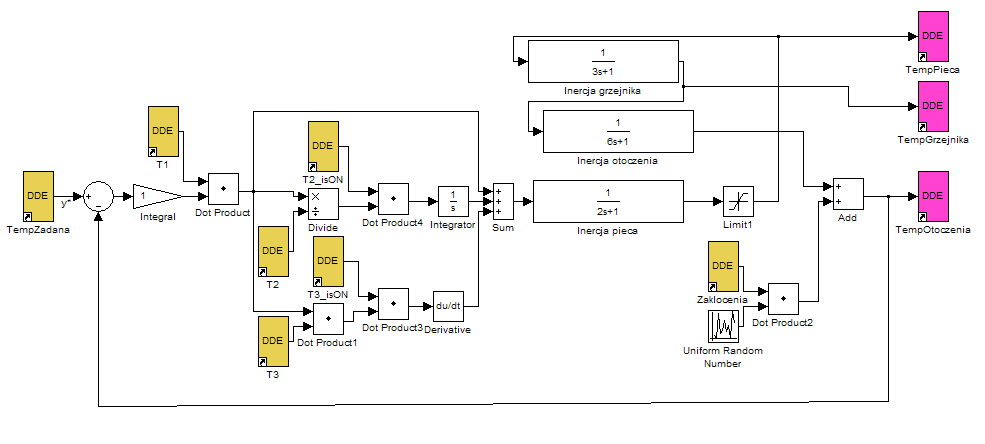
\includegraphics[width=120mm]{CW6-model.png}
	\caption{Schemat modelu systemu sterowania z Simulinka.}
    \label{fig:Rysunek}
\end{figure}
\begin{figure}[!h]
    \centering
	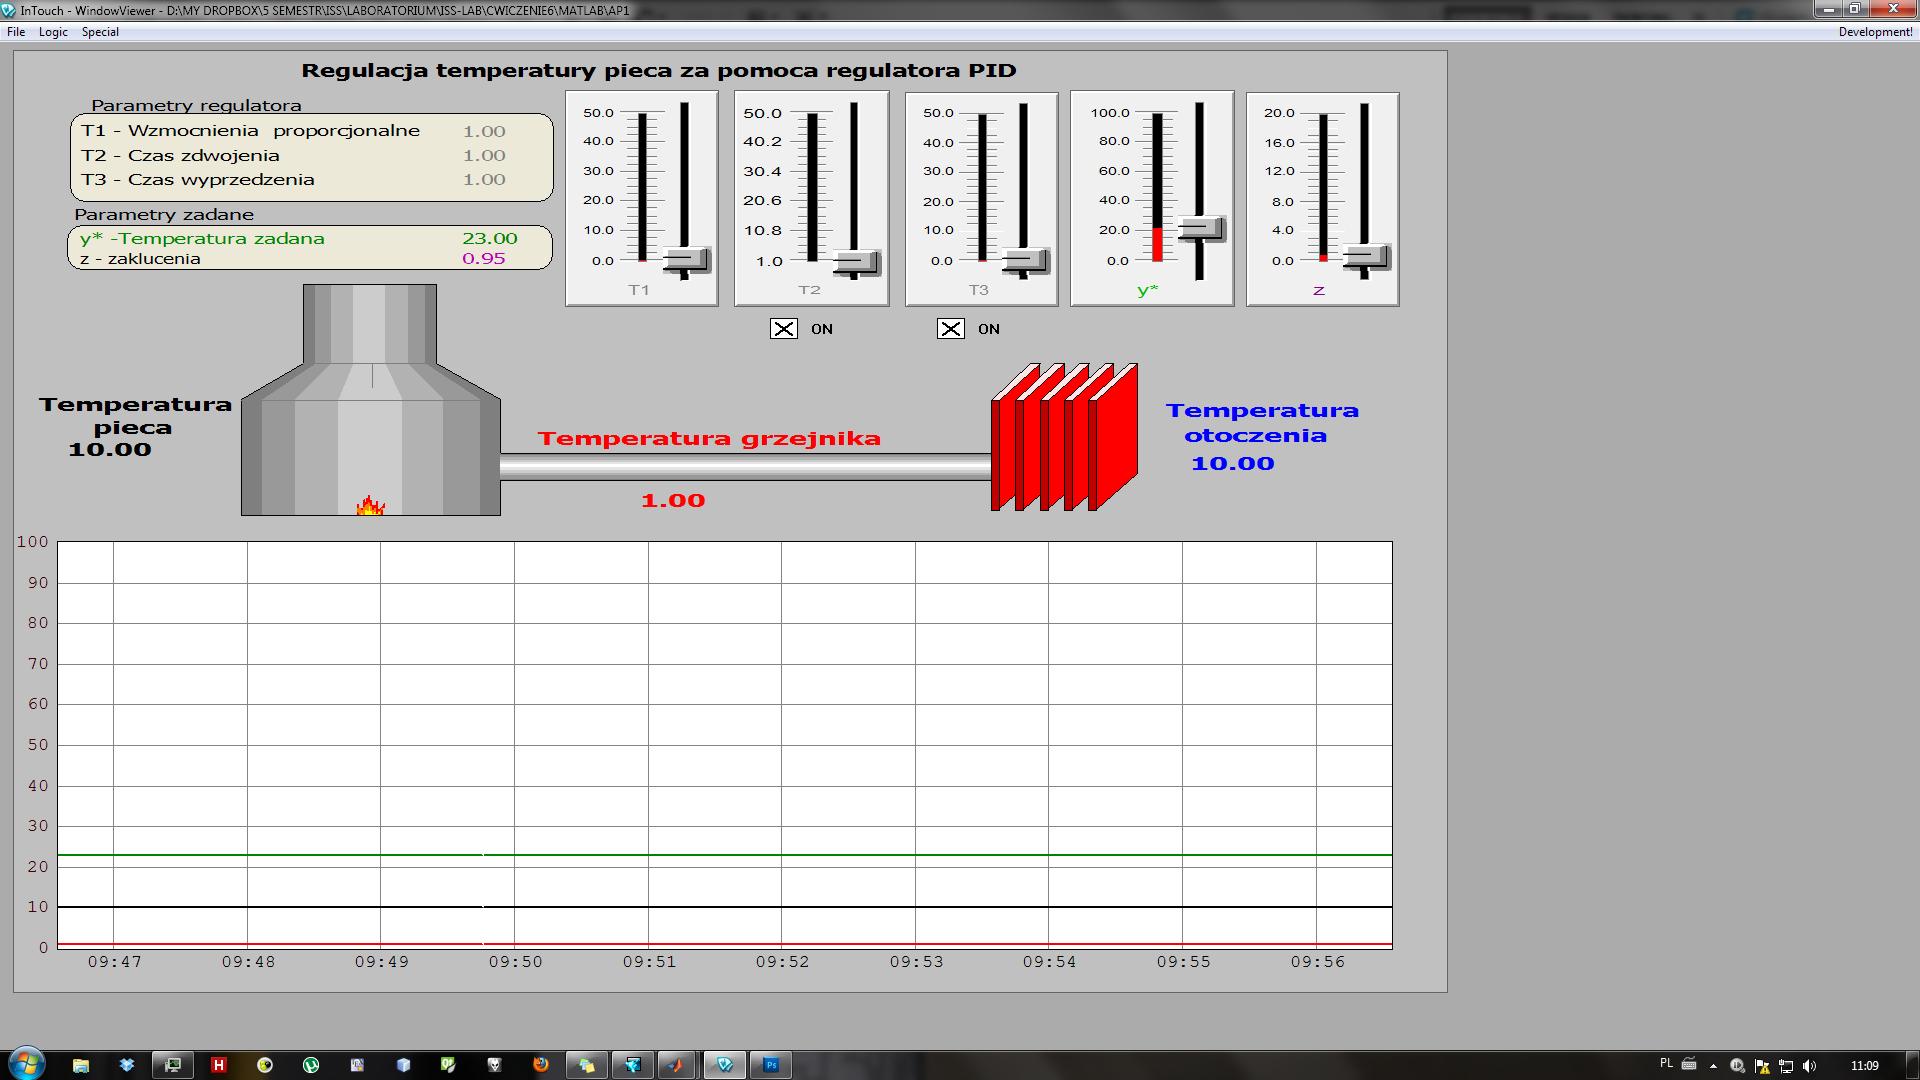
\includegraphics[width=120mm]{CW6-start.png}
	\caption{Screen ekranu projektu programu InTouch do symulacji systemu.}
    \label{fig:Rysunek}
\end{figure}
Na powyższym rysunku pokazany jest ekran służący nam do symulacji systemem sterowania. Suwaki w górnej części ekranu regulować będą wartości parametrów regulatora PID, wartość zadaną, oraz wielkość zakłóceń. Wykres w dolnej części ekranu będzie natomiast przedstawiał wykresy przebiegów temperatur pieca, grzejnika i otoczenia.

Aby uruchomić symulacje należy umieścić wszystkie pliki modelu Simulinka, bibliotek DDE, oraz folder z projektem programu InTouch umieścić w jednym folderze. Najpierw należy uruchomić projekt programu InTouch w trybie 'Runtime'. Następnie należy uruchomić program Matlab i model systemu sterowania z Simulinka. Ostatnią rzeczą którą należy zrobić jest uruchomienie symulacji w okienku modelu systemu sterowania. W tym momencie oba programy zaczną ze sobą współpracować, a my będziemy mogli ustawiać parametry systemu sterowania w oknie projektu InTouch.

%---------------------------------------------------------------------------------------------------------------------
%ZADANIE 2
%---------------------------------------------------------------------------------------------------------------------
\subsection{Dobór optymalnych parametrów regulatora.}\label{sec:zad2}
\begin{enumerate}
	\item Wyznaczenie K na granicy stabilności\\
		Ten etap sprawił nam spore trudności, ze względu na niedokładność suwaków i wykresu.
		\begin{figure}[!h]
		    \centering
			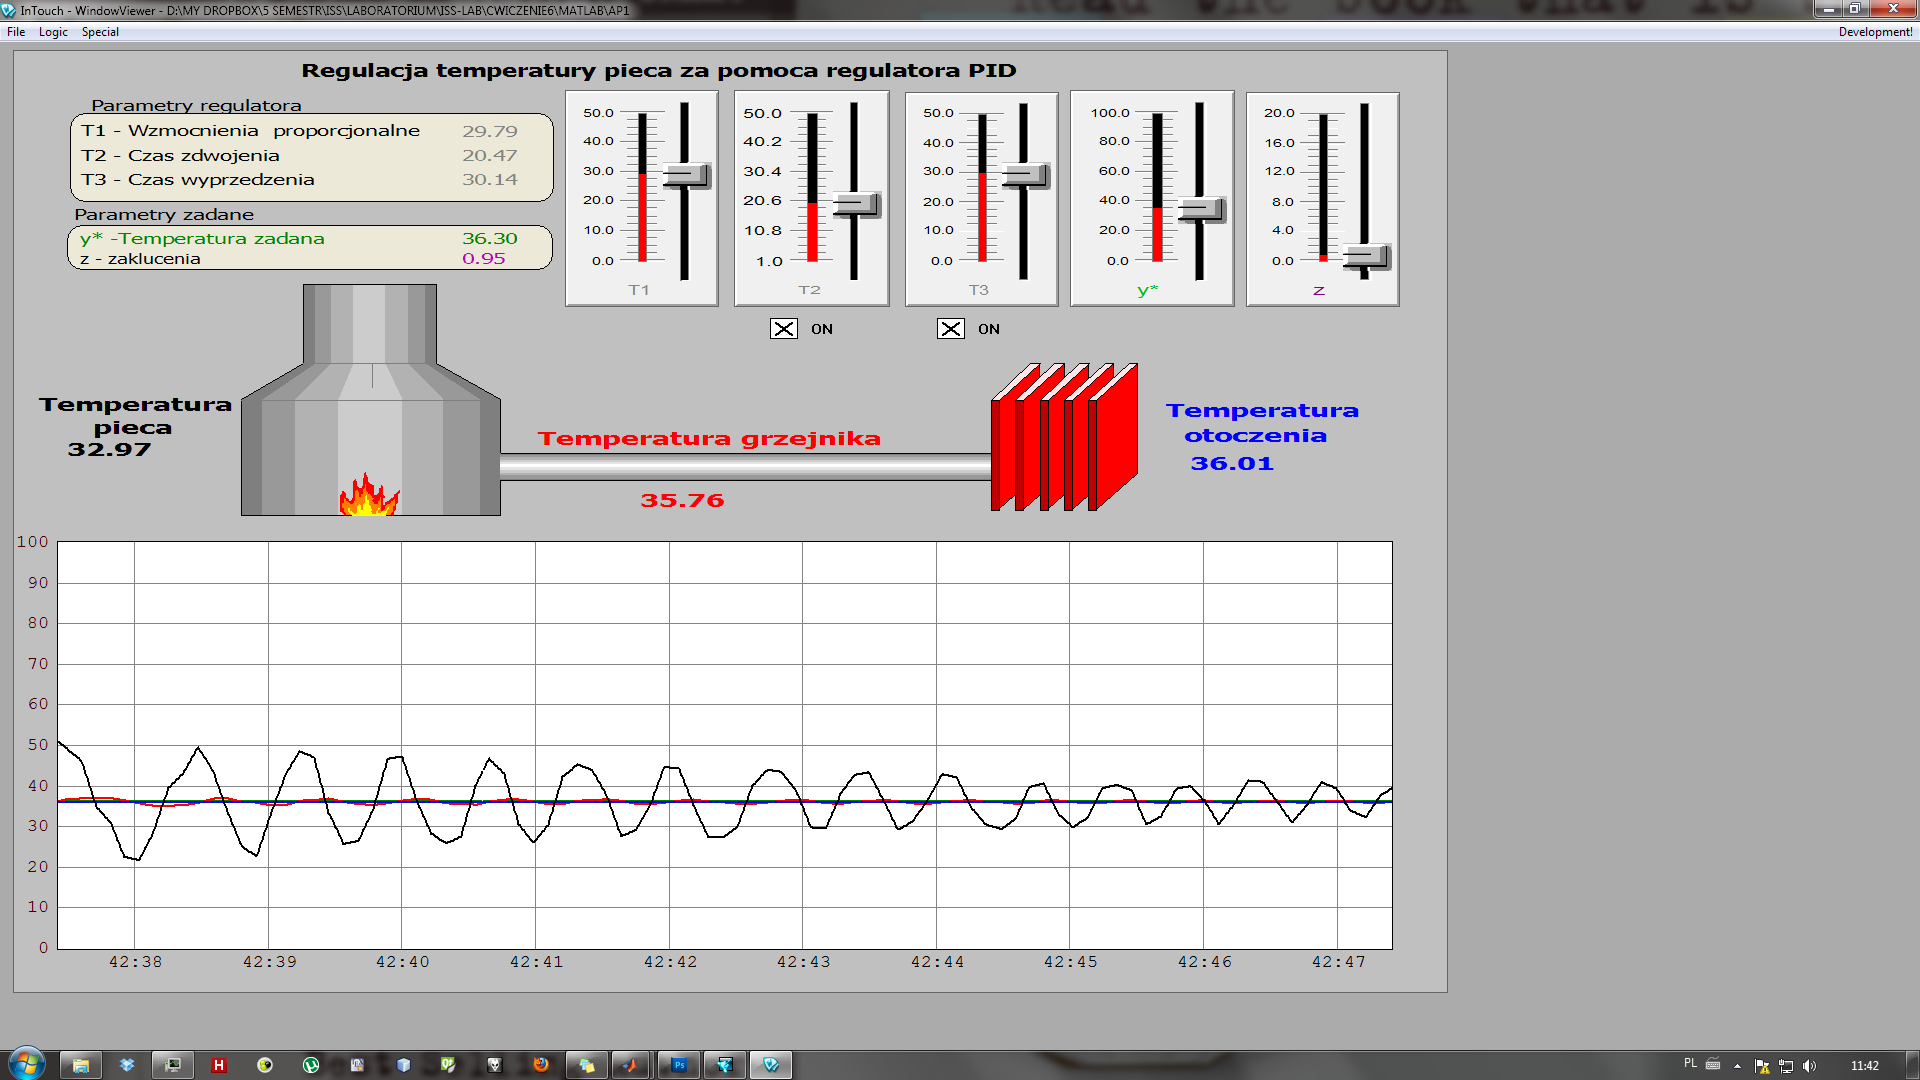
\includegraphics[width=120mm]{CW6-T130-(Kkr)-T220-T330.png}
			\caption{Wykres}
		    \label{fig:Rysunek}
		\end{figure}
		Dla nieco większych wartości otrzynaliśmy bardzo niestabilny układ.
		\begin{figure}[!h]
		    \centering
			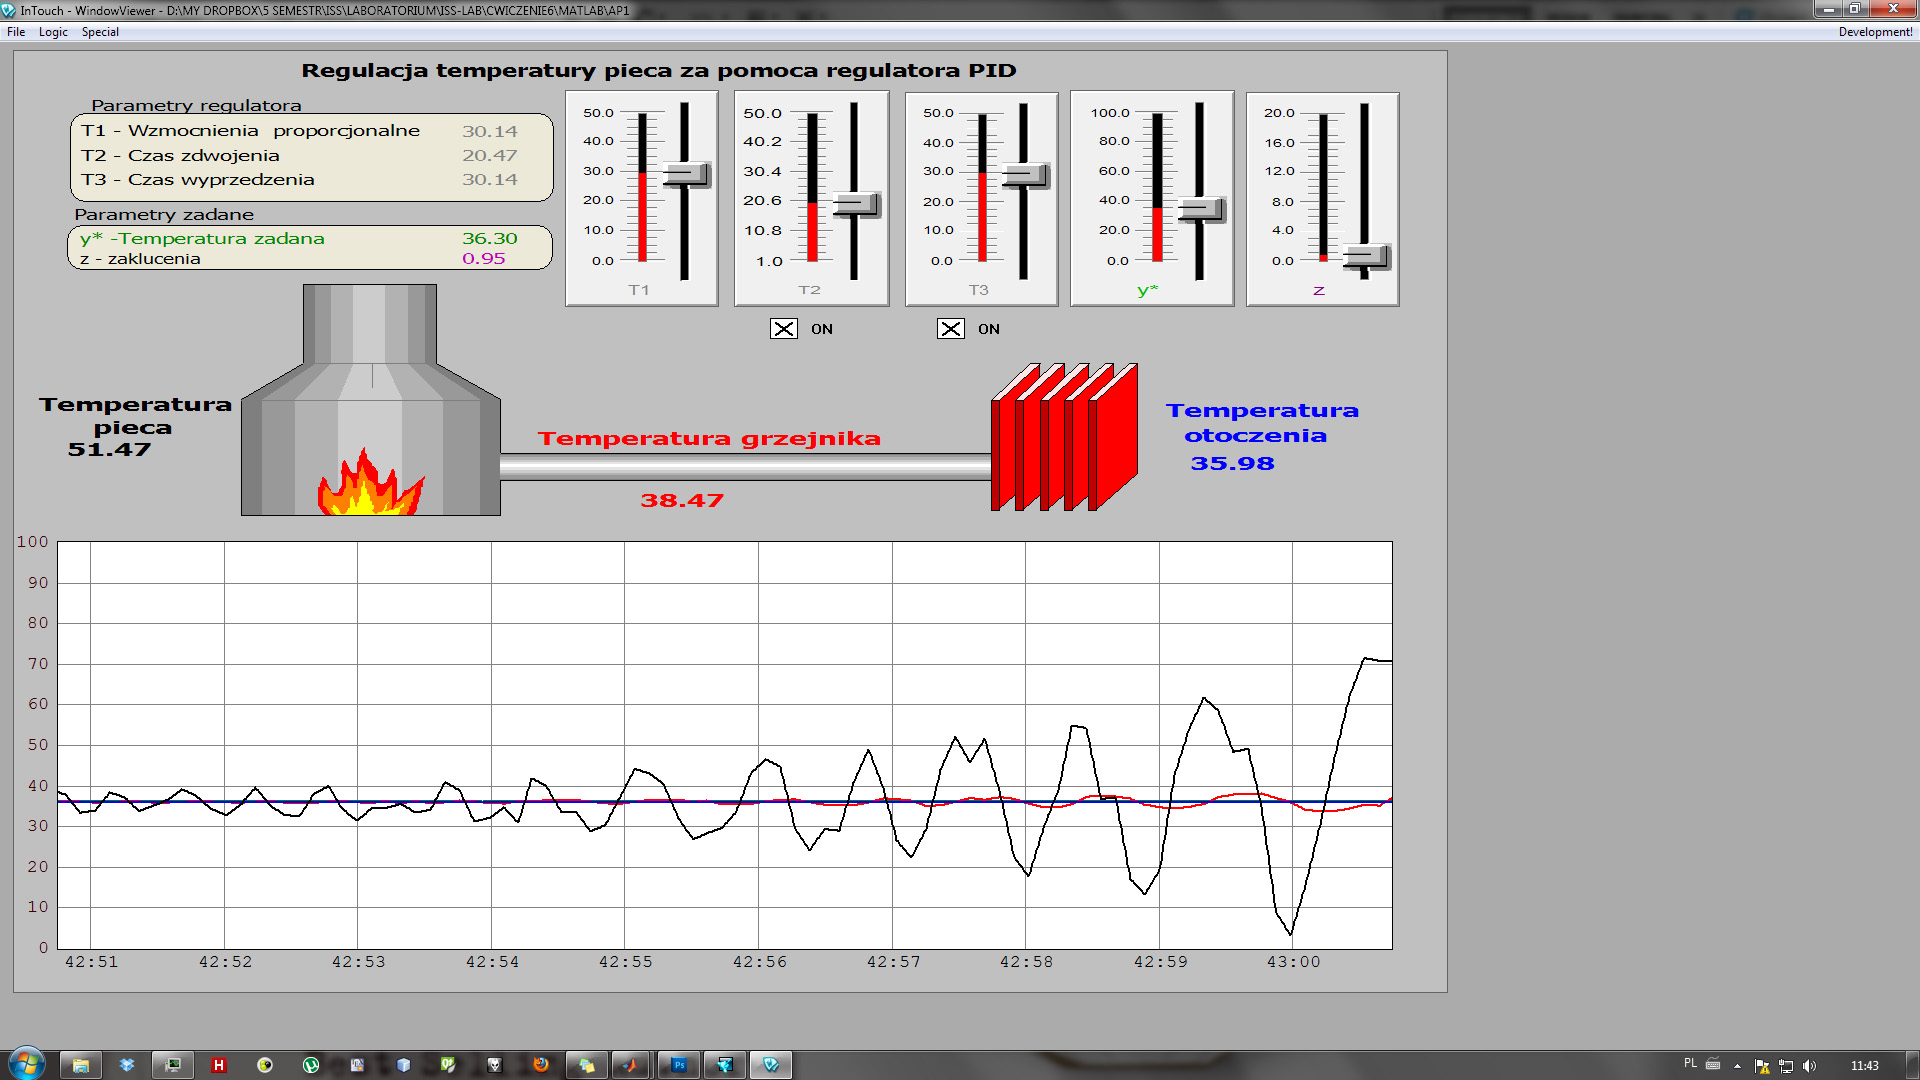
\includegraphics[width=120mm]{CW6-T130+(Kkr)-T220-T330.png}
			\caption{Wykres}
		    \label{fig:Rysunek}
		\end{figure}
		Dlatego wybraliśmy Kkr z pierwszego wykresu.\newpage
	\item Metoda Zieglera-Nicholsa	

\begin{tabular}{ | l | c | c | c | c | c | c | }
\hline
  Typ regulatora & \multicolumn{6}{|c|}{Optymalne wartości parametrów} \\   \hline
   & \multicolumn{3}{|c|}{Próba skokowa} & \multicolumn{3}{|c|}{Granica stabilności} \\   \hline
   & $K_{p}$ & $T_{i}$ & $T_{d}$ & $K_{p}$ & $T_{i}$ & $T_{d}$\\   \hline
   P & 1/a & - & - & $0.5K_{kr}$ & - & - \\   \hline
   PI & 0.9/a & $3 T_{d}$ & - & $0.45K_{kr}$ & $T_{osc}/1.2$ & - \\   \hline
   PID & 1.2/a & $2T_{d}$ & $0.5T_d$ & $0.6K_{kr}$ & $T_{osc}/2$ & $T_{osc}/8$ \\   \hline
\hline
\end{tabular}
\newline

Odczytane wartości z wykresu:\\
$Kkr=30$\\
$T_{osc}=0.625$\\
Obliczone wartości:\\
$K=15$\\
$T_{i}=0.3125$\\
$T_{d}=0.078125$\\
\end{enumerate}
Otrzymane wartości są tylko szacunkowe.

\section{Wnioski}
Ćwiczenie to jest podsumowaniem naszych wcześniejszych zadań. Mogliśmy w praktyce zobaczyć do czego stosuje się układy PID i jak wygląda symulacja naturalnych obiektów. Dużym problemem okazał się brak możliwości wpisania zadanych wartości, a wybieranie wartości suwakiem było trudne.
%Coś jeszcze dopisać
\end{document}